\section{Packet Trace Fusion}
\label{sec:fusion}

Due to the random loss nature of 802.11 PHY layer, a single sniffer may not be
able capture all the packets transmitted by the Device Under Test (DUT).
Inaccurate packet traces may cause either False Positives or False Negatives in
the verification process. To solve this problem, we first develop packet trace
fusion techniques which improve the accuracy of observations by merging the
packet traces collected from multiple sniffers. Nevertheless, we
also note that  inaccurate observation is inevitable regardless of the
number of sniffers used. We described the techniques to address this problem in
next section.

\subsection{Time Synchronization}
\label{subsec:sync}

\begin{figure}[t!]
  \centering
  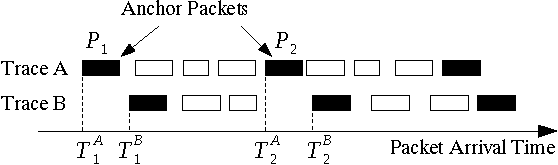
\includegraphics[width=0.48\textwidth]{./figures/sync.pdf}
  \caption{\textbf{Time Synchronization Between Two Packet Traces.}}
  \label{fig:sync}
\end{figure}

Similar to previous
works~\cite{Yeo:2004:FWL:1023646.1023660,Mahajan:2006:AMB:1159913.1159923,Cheng:2006:JSP:1159913.1159920},
we use reference packets that are unique across multiple packet traces as
\textit{anchor} packets for adjusting relative clock skew and drift. More
specifically, we use the AP beacon frames which contain a unique source MAC
address and a 64~bit Time Synchronization Function (TSF) timestamp that
increments monotonically at microsecond granularity.

\begin{figure}[t!]
  \centering
  \begin{subfigure}{0.48\textwidth}
    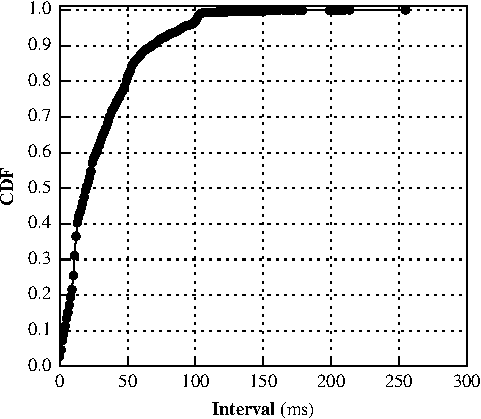
\includegraphics[width=\textwidth]{./figures/AnchorInterval.pdf}
    \caption{\textbf{CDF of Interval Between Anchor Packets.}}
    \label{fig:anchor_interval}
  \end{subfigure}
  \begin{subfigure}{0.48\textwidth}
    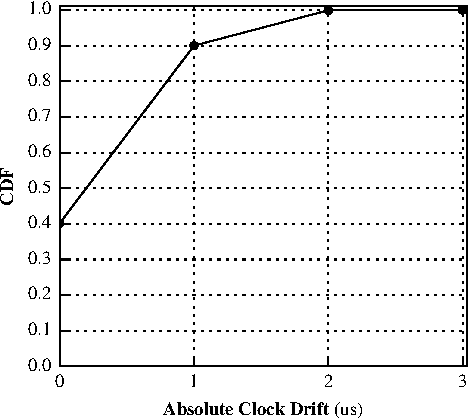
\includegraphics[width=\textwidth]{./figures/DriftRate.pdf}
    \caption{\textbf{CDF of Drifts during Consecutive Anchor Packets.}}
    \label{fig:anchor_drift}
  \end{subfigure}
  \caption{\textbf{Statistics of Time Sychronization.}}
\end{figure}

The time synchronization process of two packet traces is illustrated in
Figure~\ref{fig:sync}. The arrival time of two consecutive anchor packets at the
two packet traces are $T^A_1, T^B_1$ and $T^A_2, T^B_2$ respectively. Assume
that the relative clock drift rate of packet trace $B$ is constant during the
period between $P_1$ and $P_2$, the packet arrival timestamps of trace $B$ can
be adjusted to synchronize with trace $A$ using Equation~\ref{eqn:sync}.

\begin{align}
  T^B_{\text{new}} = \frac{T^A_2-T^A_1}{T^B_2-T^B_1}(T^B_{\text{old}}-T^B_1)+T^A_1
  \label{eqn:sync}
\end{align}

In order to avoid clock fluctuation over long durations, the above time
synchronization operation is performed independently for each sub-traces between
consecutive anchor packets. To quantify the clock drift during each anchor
interval, we define the absolute drift ($D$) as Equation~\ref{eqn:drift}.

\begin{align}
  D = |(T^B_2 - T^A_2) - (T^B_1-T^A_1)|
  \label{eqn:drift}
\end{align}

Intuitively, the smaller the absolute drift during the anchor interval, the more
likely the linear drifting rate assumption holds true.

To evaluate the feasibility and accuracy of the time synchronization method,
we obtained two real world packet traces in an office environment. Both traces
contains about 522~K packets collected during 10 minutes. In total, we found
\num{16796} anchor packets (common beacon packets) from the two packet traces, and
Figure~\ref{fig:anchor_interval} shows the CDF of the interval between two
consecutive anchor packets. The 99 percentile is at around 100 ms, which
aligns with the typical beacon interval. Figure~\ref{fig:anchor_drift}
shows the CDF of absolute drift during each anchor intervals. The maximum clock
drift is 3~\us{}, which is far less than the 802.11 slot time (9~\us{}). These
statistics show that it is feasible to perform accurate time synchronization
between the packet traces collected from multiple sniffers.

\subsection{Packet Trace Merging}

Having synchronized the timestamps between packet traces, we next merge multiple
traces to obtain more accurate observation. Similar to time synchronization,
packet merging is performed independently for each sub-traces between two
consecutive anchor packets, then the merged sub-traces are concatenated together
to form the final merged trace. The algorithm to merge two sub traces is shown
in Algorithm~\ref{algo:merge}.

\begin{algorithm}[t!]
  \caption{Merging two synchronized sub-traces.}
  \label{algo:merge}
  \begin{algorithmic}[1]
    \Require{$subtrace1$ and $subtrace2$ are already synchronized using the
    technique described in Section~\ref{subsec:sync}.}
    \Statex
    \Function{merge}{$subtrace1$, $subtrace2$}
      \Let{all\_pkts}{\Call{concatenate}{$subtrace1$, $subtrace2$}}
      \Let{merged}{[]}
      \Let{last\_pkt}{$nil$}
      \For{pkt \textbf{in} \Call{sorted}{all\_pkts}}
        \If{last\_pkt == $nil$ \textbf{or}
            \State (pkt.ts - last\_pkt.ts > $THRES$) \textbf{or}
            \State \Call{hash}{pkt} $\ne$ \Call{hash}{last\_pkt}}
          \State \Call{append}{merged, pkt}
        \EndIf
        \Let{last\_pkt}{pkt}
      \EndFor
    \EndFunction
  \end{algorithmic}
\end{algorithm}

Two packets from difference packet traces are identified as distinct if either
their synchronized timestamps are at least $THRES$ apart (line 7) or their raw
content differs (line 8).  Based on the results in
Figure~\ref{fig:anchor_drift}, we choose $THRES$ to be 4~\us{} in following
evaluations. We use the waterfall merging process proposed by R. Mahajan
\textit{et al}~\cite{Mahajan:2006:AMB:1159913.1159923} to merge multiple traces.

To evaluate the effect of packet fusion in reducing missing packets from DUT, we
first instrument the Minstrel rate control algorithm in Linux \texttt{mac80211}
framework to obtain the retry chain of each transmitted packet. An example retry
chain of a packet looks like this:

\begin{verbatim}
  227 96:6 108:6 96:6 2:3
\end{verbatim}

This means the packet of sequence number 227 was transmitted 6 times at 48~Mbps,
6 times at 54~Mbps, 6 times at 48~Mbps and finally 3 times at 1~Mbps. Such
information gives us the exact number of packets transmitted by the DUT. We
then define the \textit{quality} of a packet trace as the percentage of packets
that are sent by DUT and also present in the packet trace.

We placed three sniffers near the DUT\footnote{The average RSSI of the DUT at
each sniffers is -37~dBm.} and set up the DUT to transmit 100~K
1500-bytes packets at each 802.11g bit rate. For each bit rate, we calculate the
quality of merged trace from 1, 2 and 3 sniffers respectively.
Figure~\ref{fig:quality} shows the results. We observe that for all bit rates,
the trace quality increases as the number of sniffers, especially for the high
bit rates where the packet loss probability individual sniffer are higher than
lower bit rates. The results suggest that using multiple sniffers can indeed
improve capture quality.

\begin{figure}[t!]
  \centering
  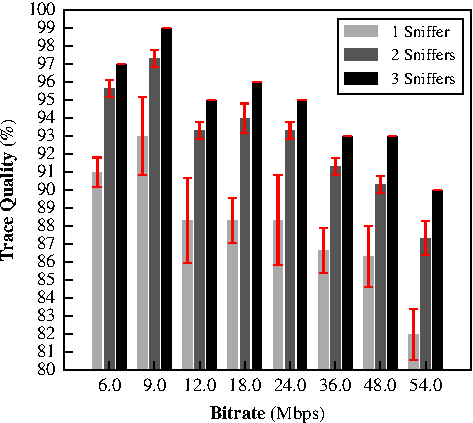
\includegraphics[width=0.48\textwidth]{./figures/CaptureQualityFigure.pdf}
  \caption{\textbf{Packet Trace Quality of Different Number of Sniffers.} Note
  that the Y-axis starts at 80\%.}
  \label{fig:quality}
\end{figure}
